\section{Fixed-Priority Scheduler}
\subsection{Purpose}
Currently, there are no systems in place within DocetOS to control the order of task execution. All tasks are treated with equal priority in relation to task execution and resource allocation. While this is acceptable for basic system usage, in real-time operation systems (RTOS), it is important for a task to be capable of meeting strict task deadlines when necessary.\hfill\newline
By implementing Fixed-Priority Scheduling in DocetOS, we allow prioritising execution of critical, time sensitive tasks above regular tasks and the preferential assignment of resources to tasks, without the complex overheads that come with implementing Dynamic-Priority Scheduling. Additionally, Priority Scheduling increases the operating systems responsiveness to external inputs such as button presses or timer triggers that require immediate response from the system.

\subsection{Specification and Design Considerations}
\subsubsection{Task Priority}
Tasks in the embedded system need to be assigned priorities based on their importance and timing requirements. Priorities must be assigned on initialisation and remain static throughout runtime, unless mutex priority inheritance is triggered. Higher-priority tasks must be scheduled to run before lower-priority ones, ensuring timely execution of time-sensitive processes. Where two tasks share the same priority, they need to operate in round-robin. The number of priority levels must be configurable through a system definition.

\subsubsection{Pre-emption}
To handle tasks with varying execution times, the fixed-priority scheduler must support pre-emption. When a higher-priority task becomes ready to run, it will pre-empt the currently executing task, interrupting the lower-priority task allowing shorter response times to critical higher-priority tasks.

\subsubsection{Task Synchronisation}
To aid task synchronisation mechanisms within the system such as semaphores and mutexes, the scheduler must support the movement of tasks from the running task list to waiting lists and vice versa. When notifying tasks and returning them to the task list, checks must be in place to verify task priority and ensure pre-emption triggers where necessary.

\subsection{Implemented Design and Functionality}
\subsubsection{Scheduler Data Structure}
\begin{center}
	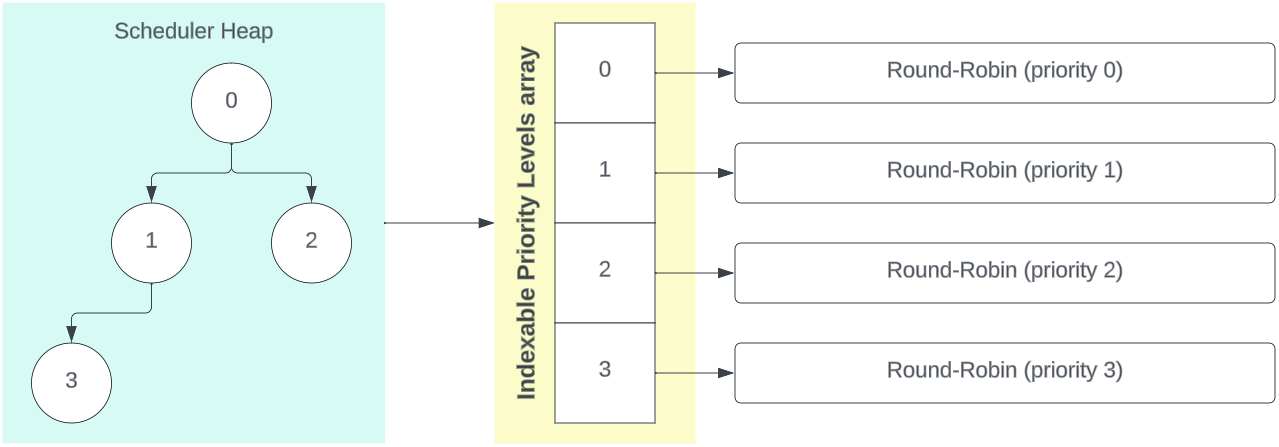
\includegraphics[width=1\textwidth]{scheduler.png}
\end{center}
In adapting the initial round-robin structure to support fixed-priority scheduling, we replicate the round-robin for each priority level, akin to a bucket queue. This allows indexing priority levels with a time complexity of O(1) instead of linearly searching for specific priorities in a regular ordered queue. Traditionally, a bucket queue includes a pointer to the highest-priority level with a task. However, this approach necessitates a linear search through the priority levels array when extracting the highest-priority task, to find the next highest-priority level containing a task. \hfill\newline
To enhance efficiency and eliminate the need for this search, we employ a binary min-heap. The min-heap tracks priority levels in the scheduler that contain tasks. Upon removing the highest-priority task, instead of searching the priority list, we identify the next highest priority level by extracting the root of the min-heap.

\subsubsection{Scheduler Initialisation}
\begin{center}
	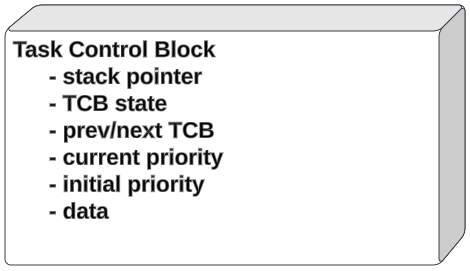
\includegraphics[width=0.5\textwidth]{tcb.png}
\end{center}
Before initiating the operating system, the scheduler is preloaded with all tasks to be executed by the user, up to a maximum task limit defined within the scheduler header file. Tasks are added to Task Control Blocks (TCBs) which are initialised with a fixed priority that remains constant throughout runtime, with the exception of when influenced by mutex priority inheritance. The priority of the TCB is constrained within the range defined by the number of priority levels specified by the OS.\hfill\newline
TCB priority is represented by an unsigned integer, with zero indicating the highest priority. Priority decreases as the integer value increases, up to the defined limit of priority levels. This design allows assigning a priority of zero to system-critical tasks, ensuring they always hold the highest priority. Increasing the number of priority levels does not then require adjusting the priority of these critical tasks since, at priority zero, they consistently remain at the highest priority, regardless of the total number of priority levels. 
 
\subsubsection{Context Switching}
In the context switch process, several safety checks facilitate the smooth operation and transition between tasks. Firstly, any priority levels devoid of tasks are pruned from the scheduler heap to prevent repetitive polling of the priority level to verify it is empty. Subsequently, the highest priority level containing tasks is retrieved from the heap using a peek operation.\hfill\newline
To conclude the context switch, the head of the highest priority level is incremented, introducing round-robin behaviour within the priority level if multiple tasks exist at the level, and the new head is returned for execution. 

\pagebreak
\subsubsection{Task Control Block (TCB) Management}
The below operations are implemented to move TCBs within the scheduler:
\setlength\tabcolsep{0pt}
\begin{center}
	\begin{tabularx}{1\textwidth}{ p{0.25\textwidth} p{0.75\textwidth} }
		\textbf{Task Waiting:}	& Removing a task from the scheduler and placing it in a waiting list.\\
		
		&\\
		
		\textbf{Task Notification:}	& Removing a task from the waiting list and returning it to the scheduler, interrupting the currently executing task if of higher priority.\\
		
		&\\
		
		\textbf{Task Priority \newline Modification:} 	& Changing a tasks priority by extracting it from the scheduler, updating the priority, and returning the task to the scheduler at the new priority level. \\
	\end{tabularx}
\end{center}
The binary heap operations and the scheduler add/remove functions do not have mutual exclusivity systems in place. Due to the complexity of the operations, using the instructions provided by the Cortex-M for mutual exclusion, LDREX and STREX, to safeguard these operations is unsuitable. However, a mutex cannot be used as mutex’s themselves use these operations, creating circular dependency. Therefore, these operations are implemented as SVC handler functions. The SVC interrupt halts thread mode execution and shifts the processor to handler mode to conduct the TCB movement, preventing other tasks or interrupts from clashing with the TCB management functions. When the movement completes, the processor is returned to thread mode to resume system execution.